\documentclass[superscriptaddress,onecolumn,floatfix]{revtex4-2}

\usepackage{graphicx}
\usepackage{epsfig}
\usepackage{color}
\usepackage{amssymb}
\usepackage{amsmath}
\usepackage{array}
\usepackage[loose]{units}
\usepackage[french]{babel}
\usepackage[unicode]{hyperref}
\usepackage{cleveref}
\usepackage{braket}
\usepackage[caption=false]{subfig}
\usepackage{letltxmacro}

\LetLtxMacro{\ORIGselectlanguage}{\selectlanguage}
\makeatletter
\DeclareRobustCommand{\selectlanguage}[1]{%
    \@ifundefined{alias@\string#1}
      {\ORIGselectlanguage{#1}}
      {\begingroup\edef\x{\endgroup
         \noexpand\ORIGselectlanguage{\@nameuse{alias@#1}}}\x}%
}
\newcommand{\definelanguagealias}[2]{%
  \@namedef{alias@#1}{#2}%
}
\makeatother

\definelanguagealias{fr}{french}


\begin{document}
\selectlanguage{fr}

\begin{abstract}
  Ce guide vous guide à travers les étapes nécessaires pour changer le mode du harnais homme-au-milieu (MITM) de votre unité principale entre les modes MITM et parallèle. Il s’agit d’une étape de dépannage ou de bricolage avancé. Voir aussi le \href{https://youtu.be/sWzxWfUpCfs}{guide vidéo}.
\end{abstract}
\title{Guide d'échange du mode homme du milieu de l'unité principale}
\author{Boutique de boutons Electroniq}
\email{support@electroniqbuttons.com}
% \affiliation{\GOE}
% \author{Benjamin J. McMorran}
% \email{mcmorran@uoregon.edu}
% \affiliation{\UO}
\date{\today}

\maketitle

\section{Introduction}
Le harnais de l'homme du milieu (MITM) de l'unité principale, illustré dans la figure \ref{subfig:overview:harness}, a deux modes possibles :
\begin{enumerate}
  \item l'homme du milieu ou en série \label{enum:MITM}
  \item parallèle \label{enum:parallel}
\end{enumerate}
\begin{figure}[h]
  \subfloat[]{\label{subfig:overview:harness}
  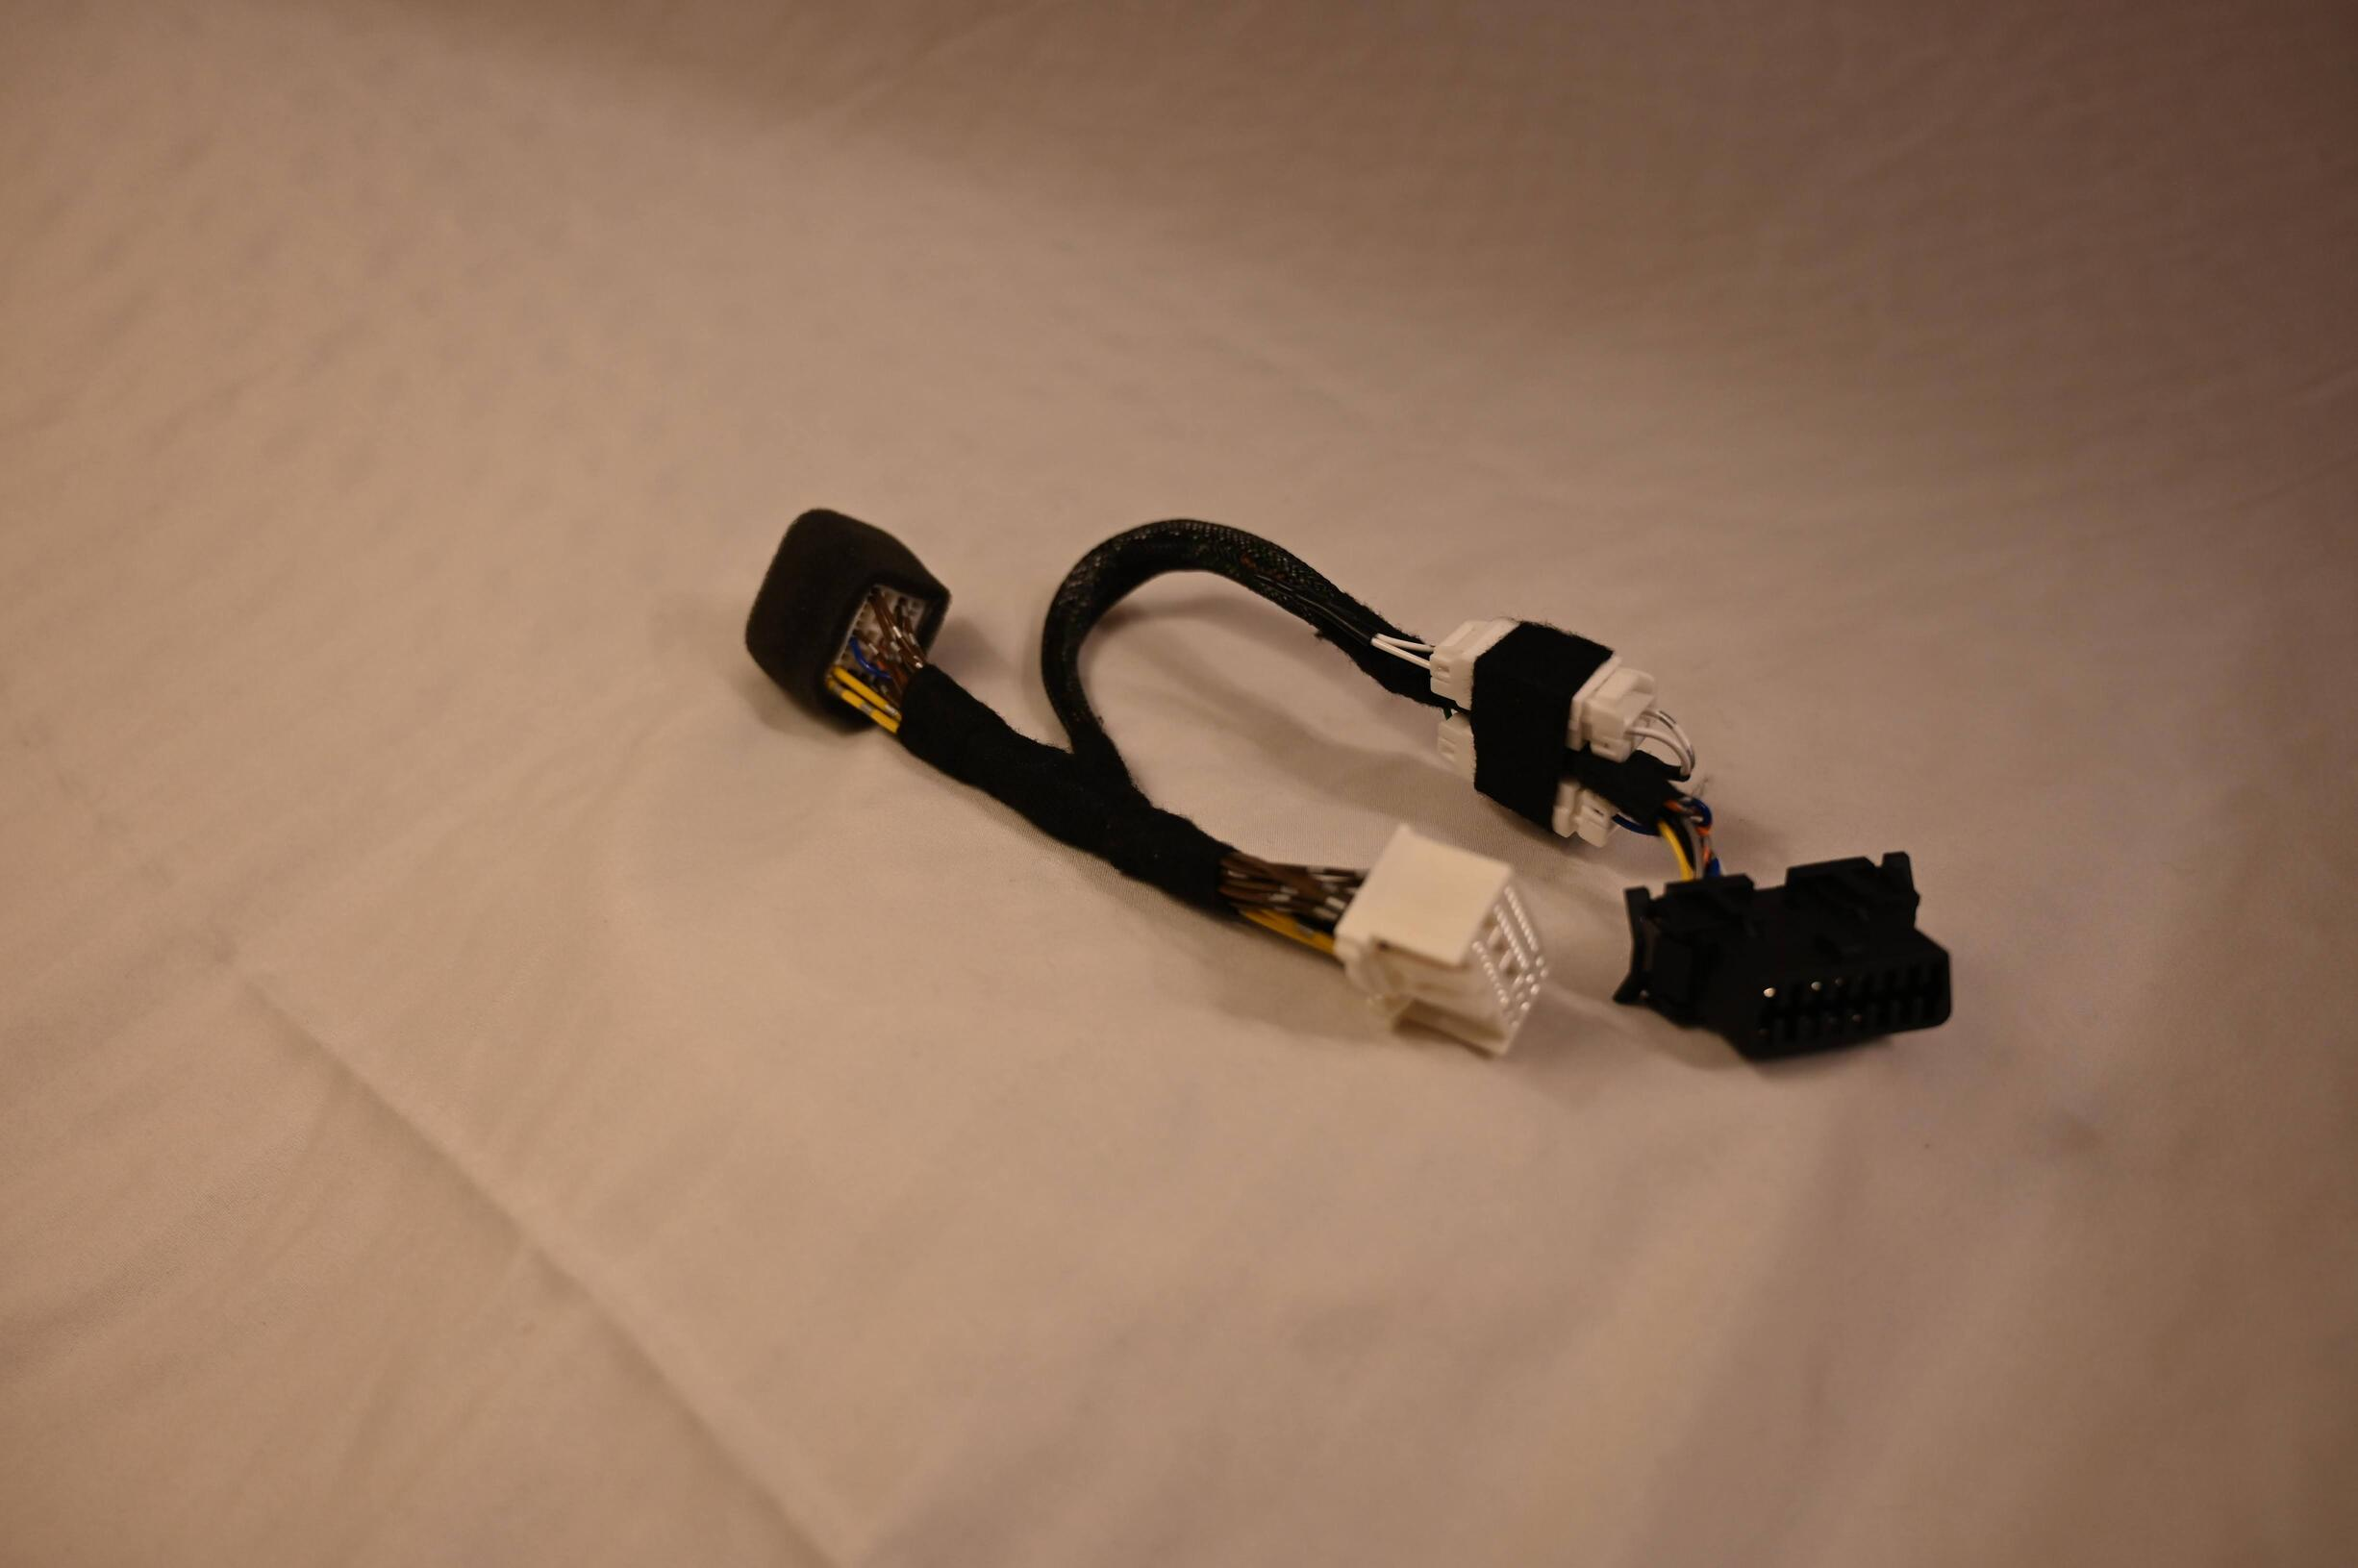
\includegraphics[height=1.95in]{photos/whole_harness.jpg} }
  \subfloat[]{\label{subfig:overview:shunt_cap_labeled}
  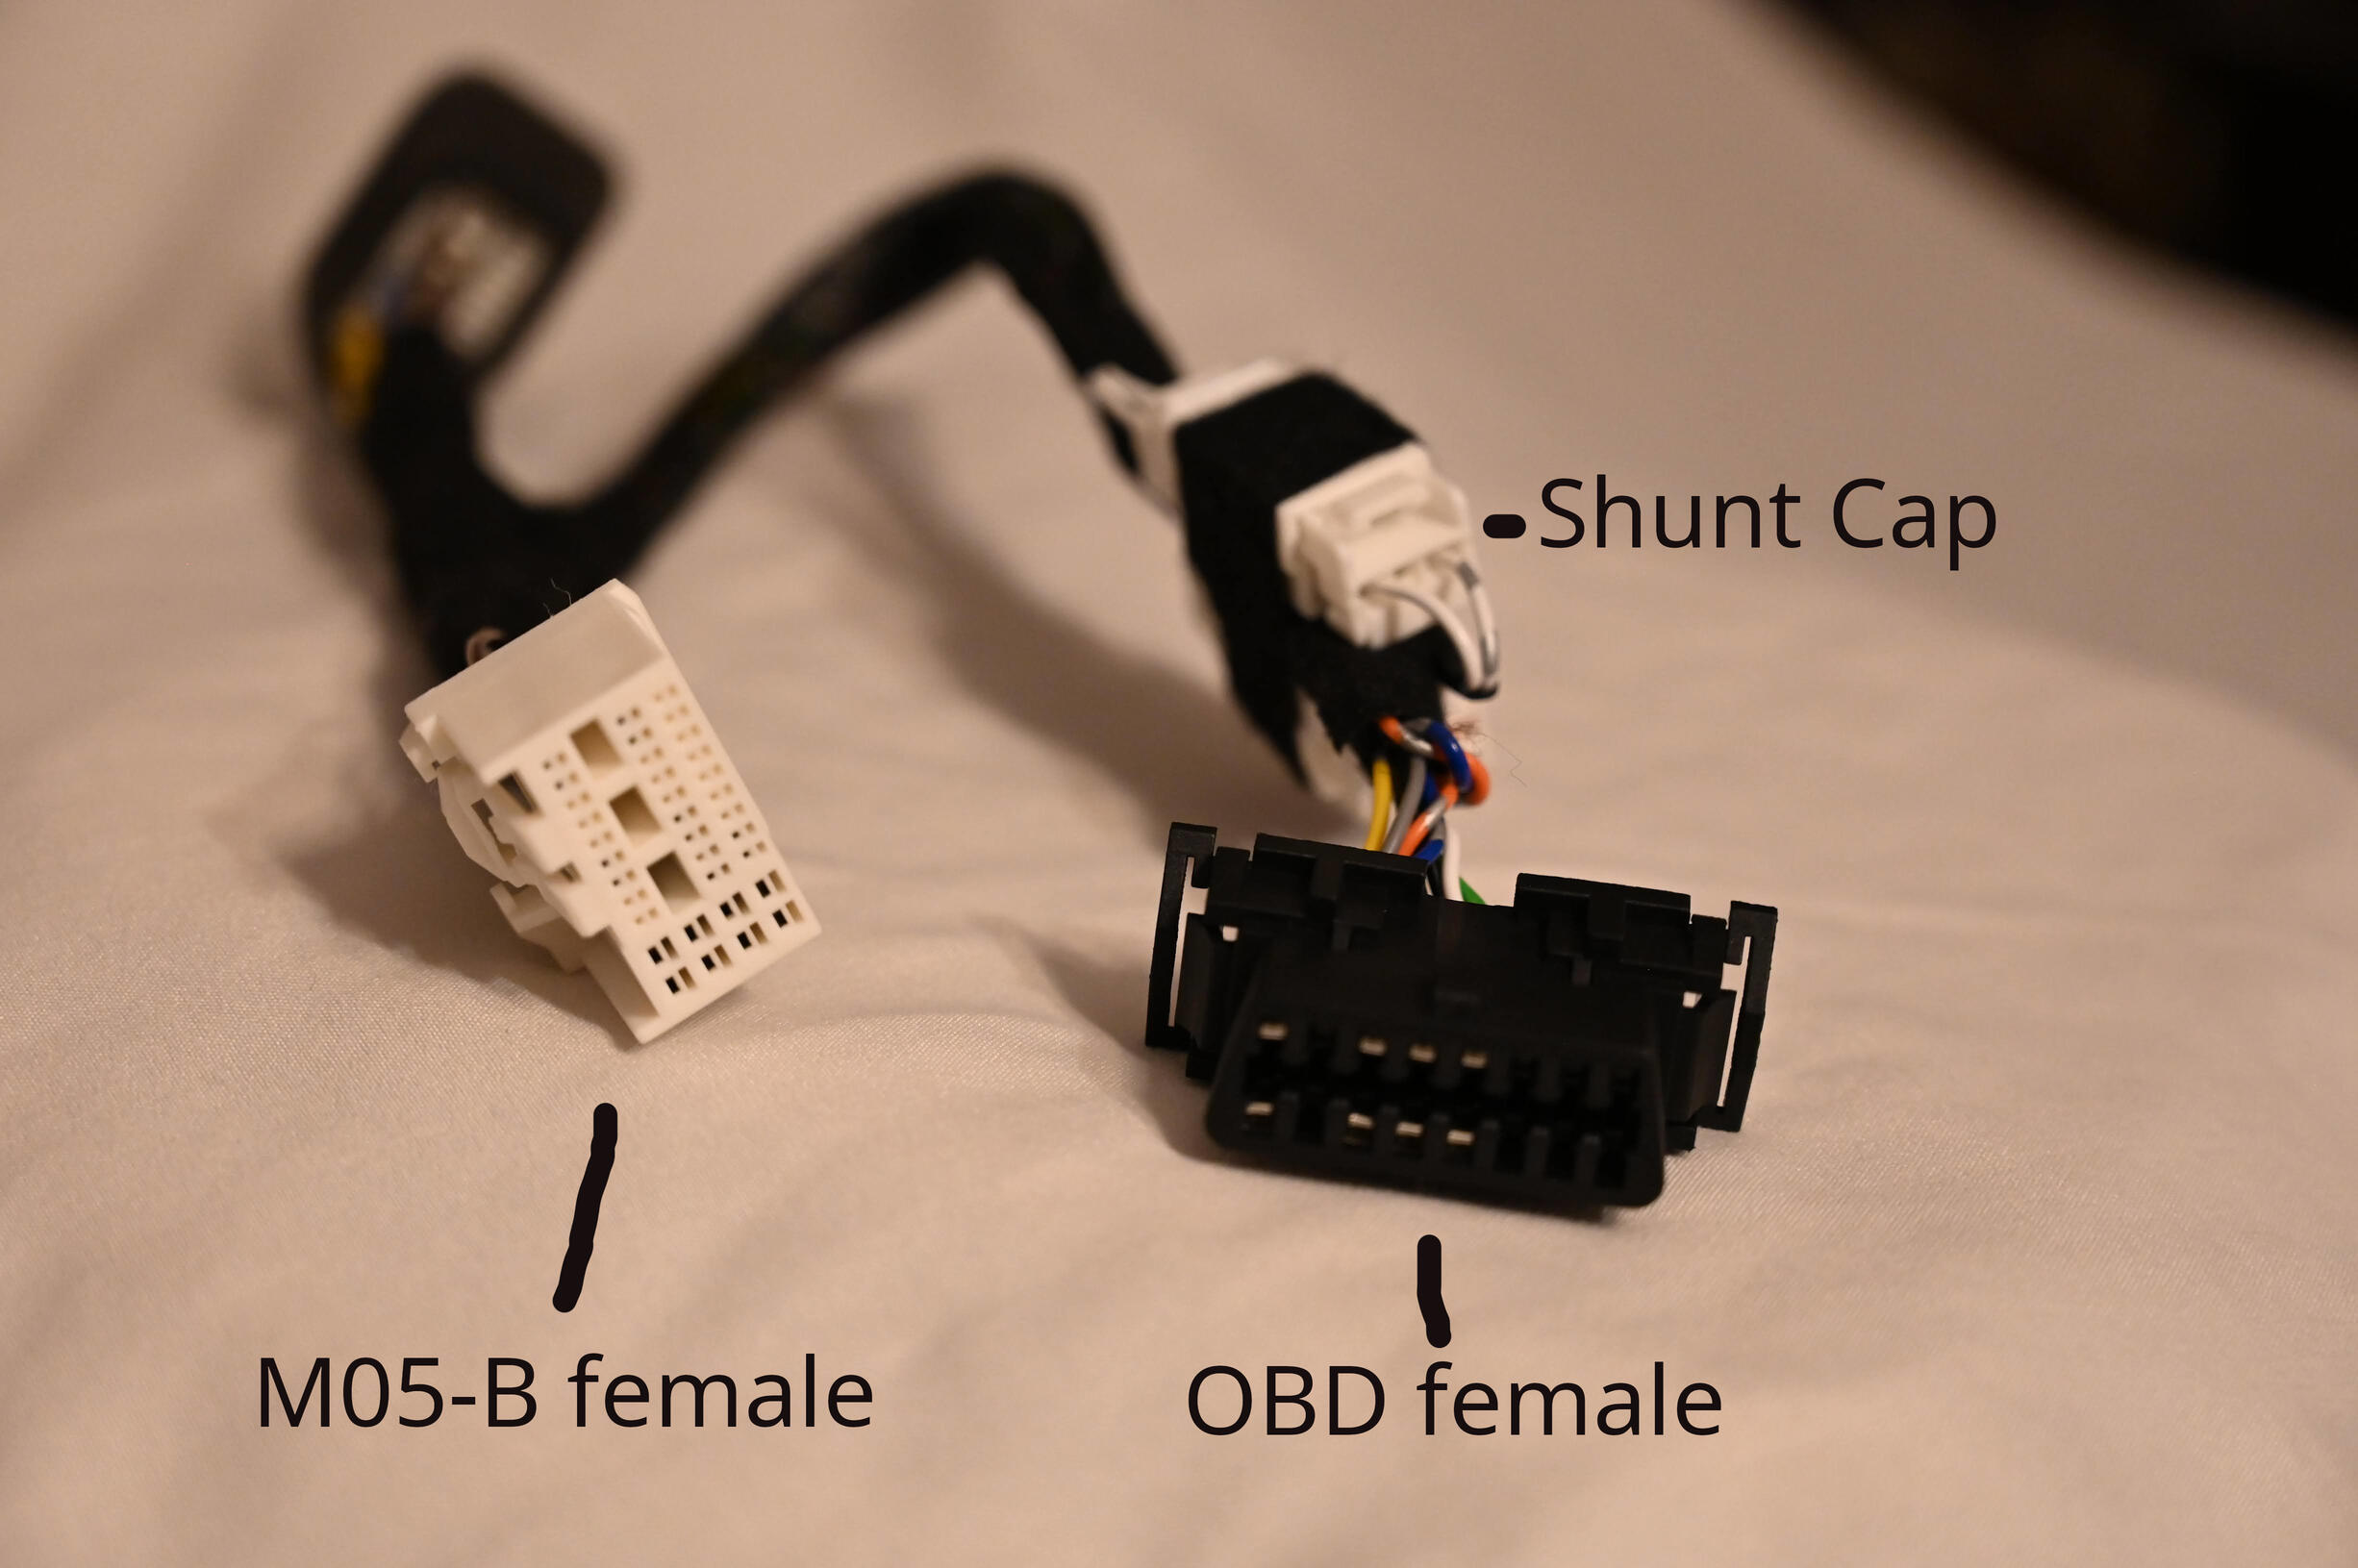
\includegraphics[height=1.95in]{photos/labeled_connectors_MITM_harness.jpg} }
   \caption{(a) Harnais d'homme au milieu. (b) Vue d'ensemble des connecteurs montrant le capuchon de shunt. \label{fig:overview}}
\end{figure}
En mode homme du milieu, les lignes de communication CAN pour l'unité principale et la voiture sont physiquement déconnectées, et un microcontrôleur branché sur le port OBD est utilisé pour transmettre sélectivement les messages entre les deux. En mode parallèle, les lignes de communication CAN sont connectées normalement et les deux jeux de broches CAN sur le port OBD sont identiques et connectés à la fois à la voiture et à l'unité principale. Le microcontrôleur se trouve sur le bus CAN de la même manière que de nombreux calculateurs sont connectés : en parallèle, il est capable d'envoyer et de recevoir des messages qui sont partagés avec tous les calculateurs du bus. 

Le harnais est conçu pour être utilisé principalement en mode MITM, mais le mode parallèle est prévu pour plusieurs raisons :
\begin{enumerate}
  \item dépannage
  \item compatibilité
\end{enumerate}
Si, par exemple, le MITM tombe en panne, vous pouvez facilement passer en mode parallèle et continuer à utiliser votre unité principale normalement sans désinstaller le harnais. De plus, certains microcontrôleurs n'ont qu'un seul jeu de broches CAN et ne peuvent pas effectuer de transfert. Le mode parallèle est fourni pour des raisons de compatibilité dans ces cas.

\section{Comment changer}
Pour changer, il vous suffit d'échanger le shunt femelle et les capuchons de shunt, qui se trouvent le plus près du port OBD. Pour passer du MITM au parallèle, procédez comme suit :
\begin{enumerate}
  \item Vérifiez que le mode de harnais actuel est MITM (Figure \ref{subfig:shunt:MITM})
  \item Débranchez le shunt femelle (fils orange et bleu, étiquetés « B1 ») (Figure \ref{subfig:shunt:female_disconnect})
  \item Débranchez le capuchon de dérivation femelle (fils blancs, étiquetés « A2 ») (Figure \ref{subfig:shunt:cap_removed})
  \item Connectez le shunt femelle au shunt mâle (fils vert et blanc, étiquetés « A1 ») (Figure \ref{subfig:shunt:parallel})
  \item Connectez le capuchon de dérivation femelle au capuchon de dérivation mâle (fils blancs, étiquetés « B2 ») (Figure \ref{subfig:shunt:parallel})
\end{enumerate}
Pour inverser le mode, inversez simplement ces instructions !
\begin{figure}[h]
  \subfloat[]{\label{subfig:shunt:MITM}
  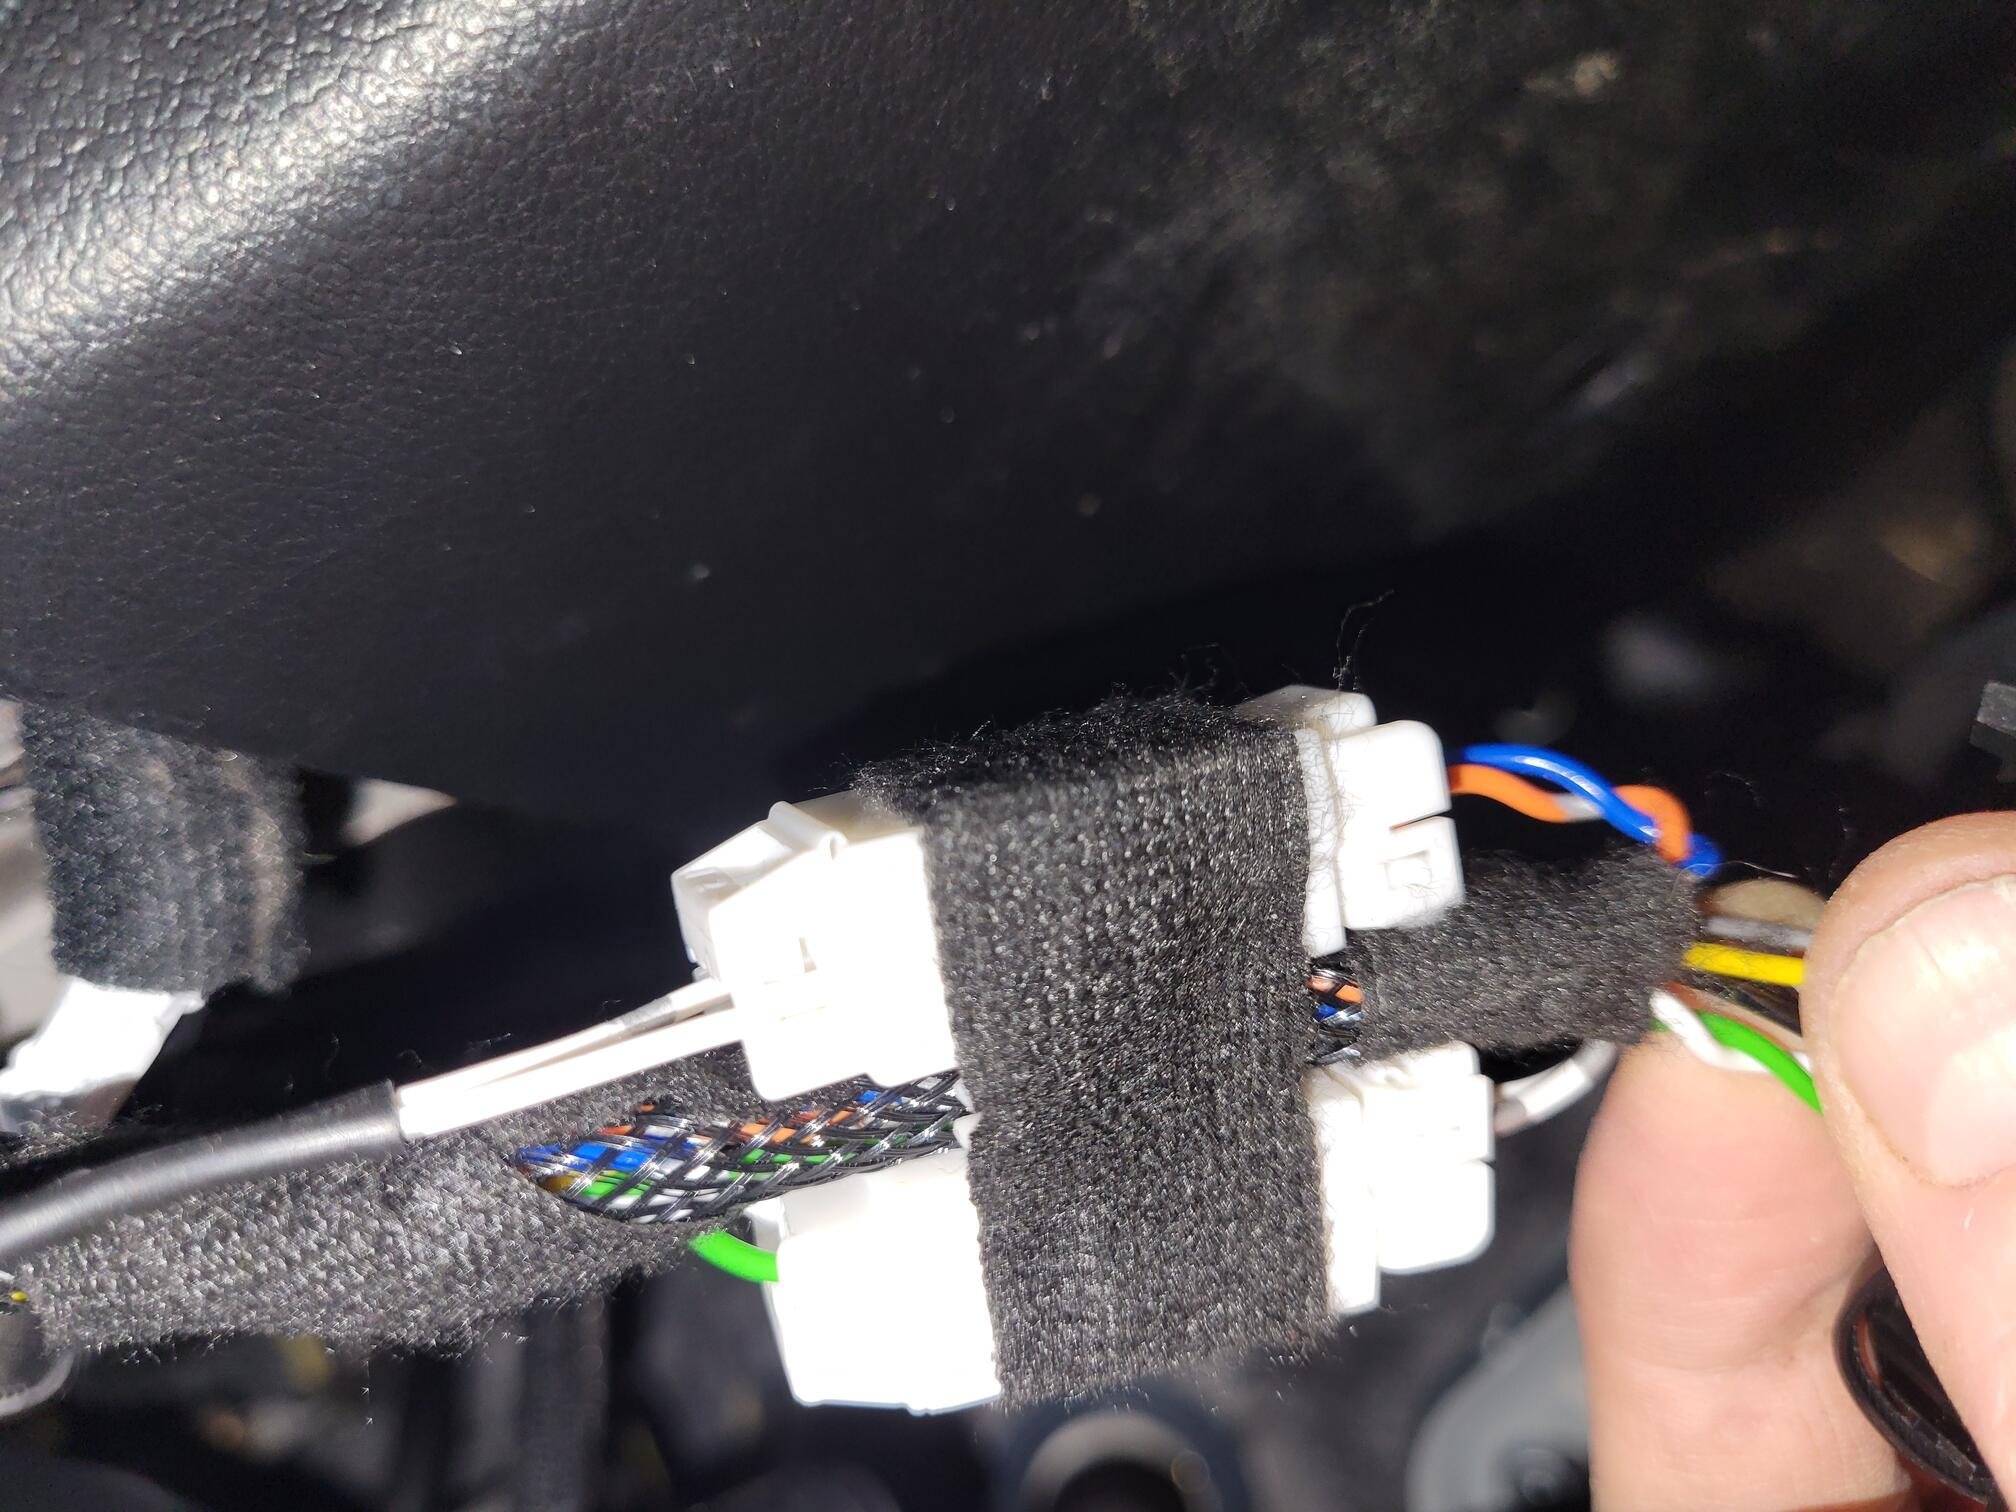
\includegraphics[height=0.95in]{photos/MITM.jpg} }
  \subfloat[]{\label{subfig:shunt:female_shunt_in_cap}
  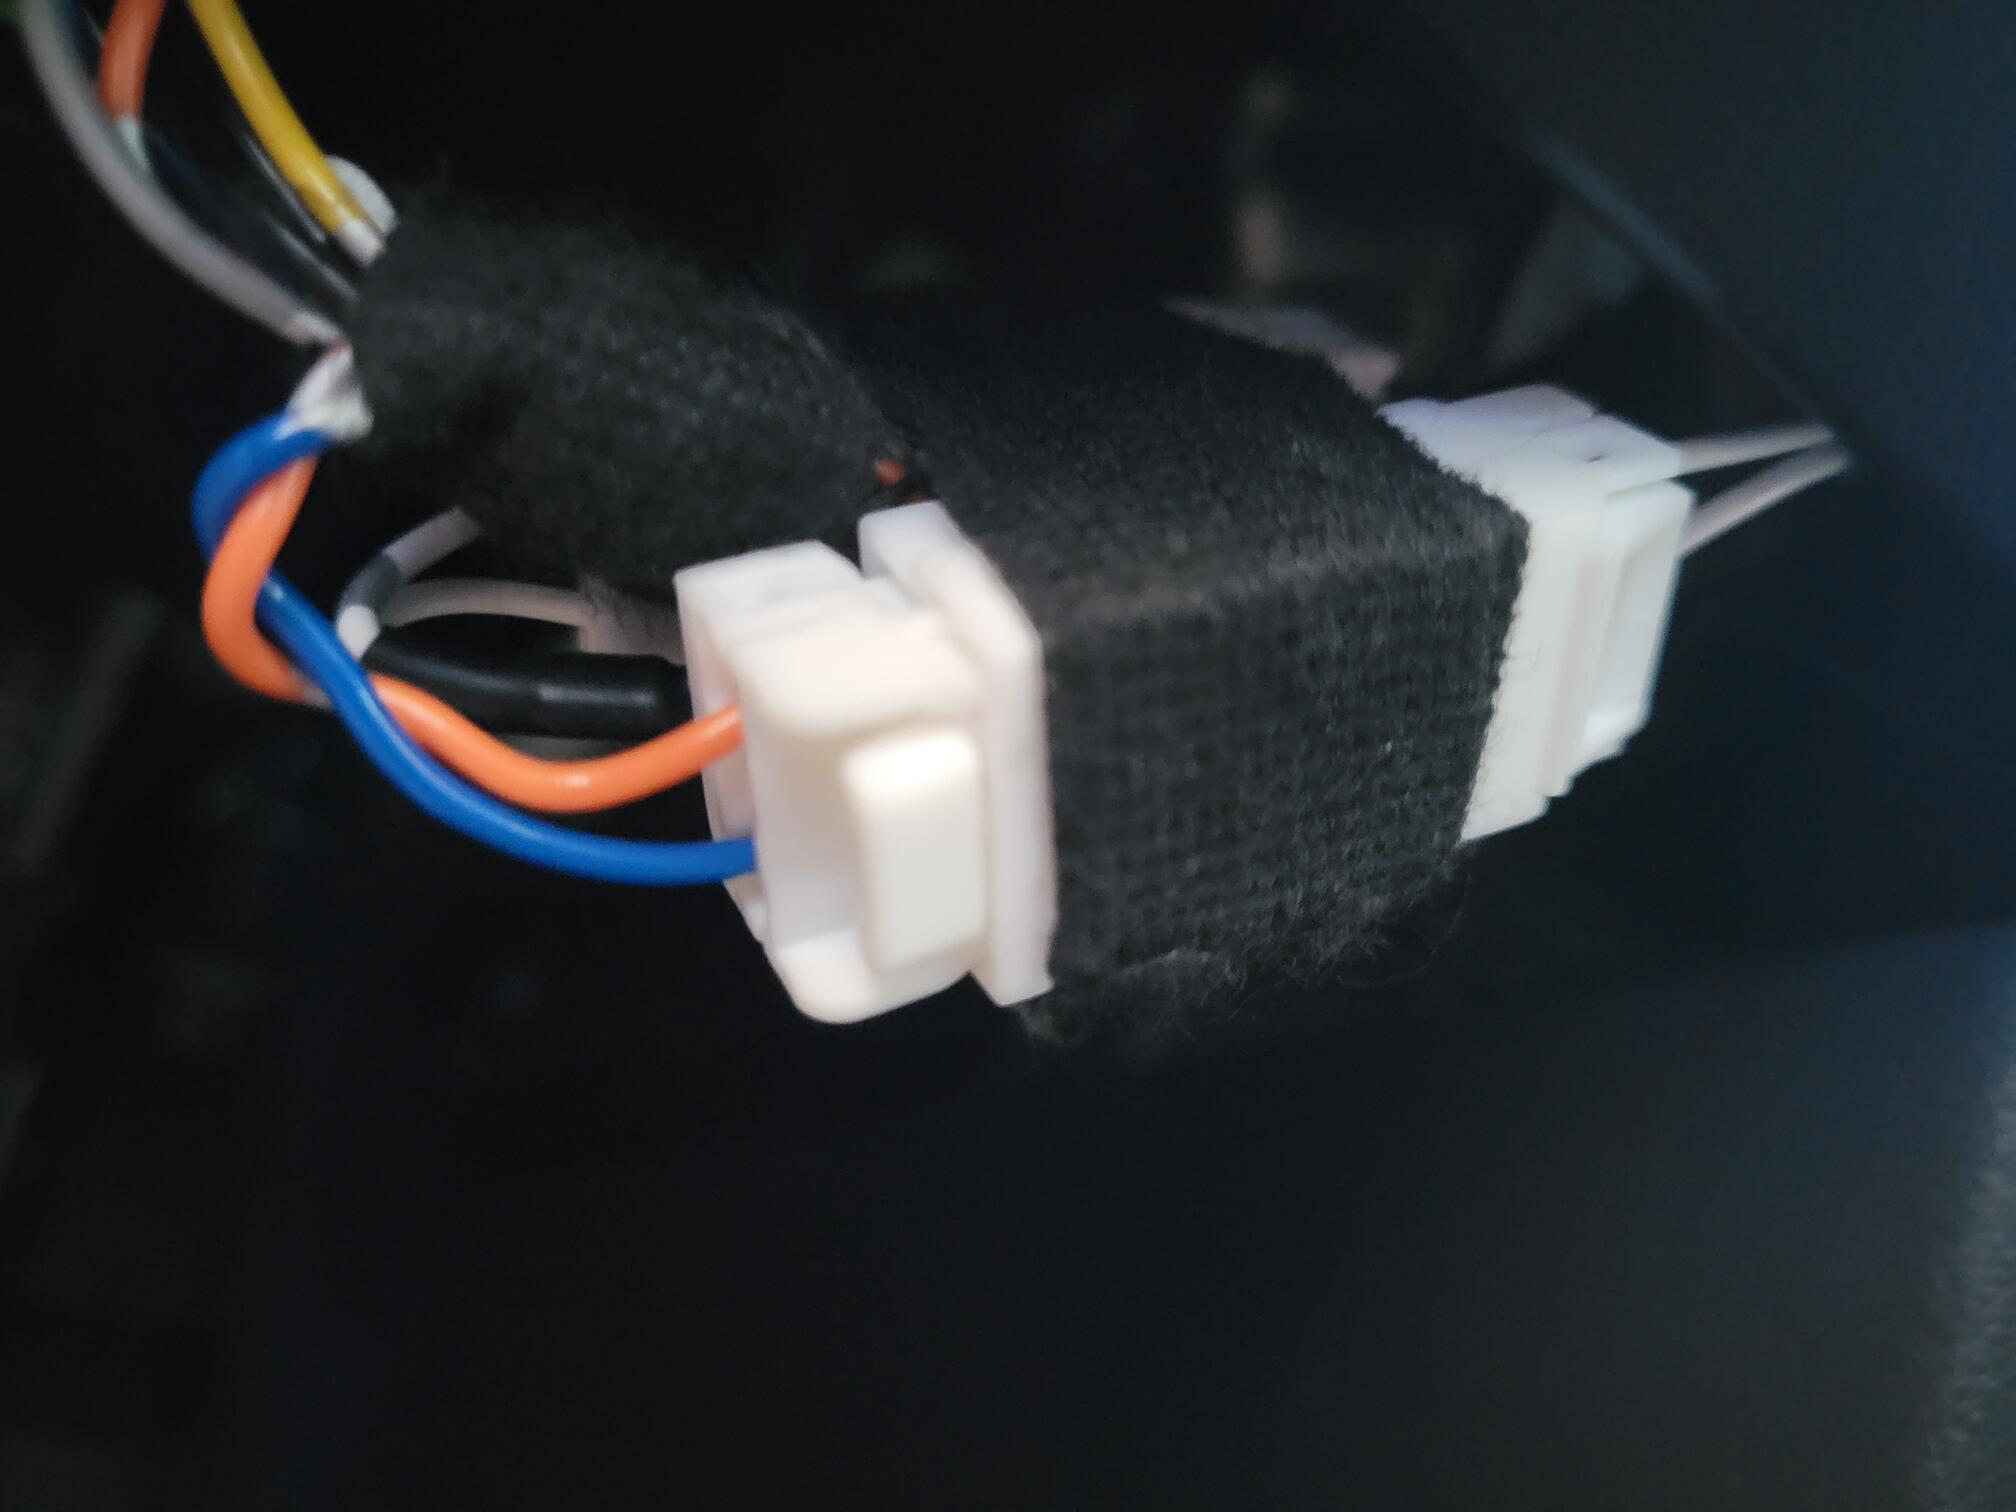
\includegraphics[height=0.95in]{photos/female_shunt_in_shunt_cap.jpg} }
  \subfloat[]{\label{subfig:shunt:female_disconnect}
  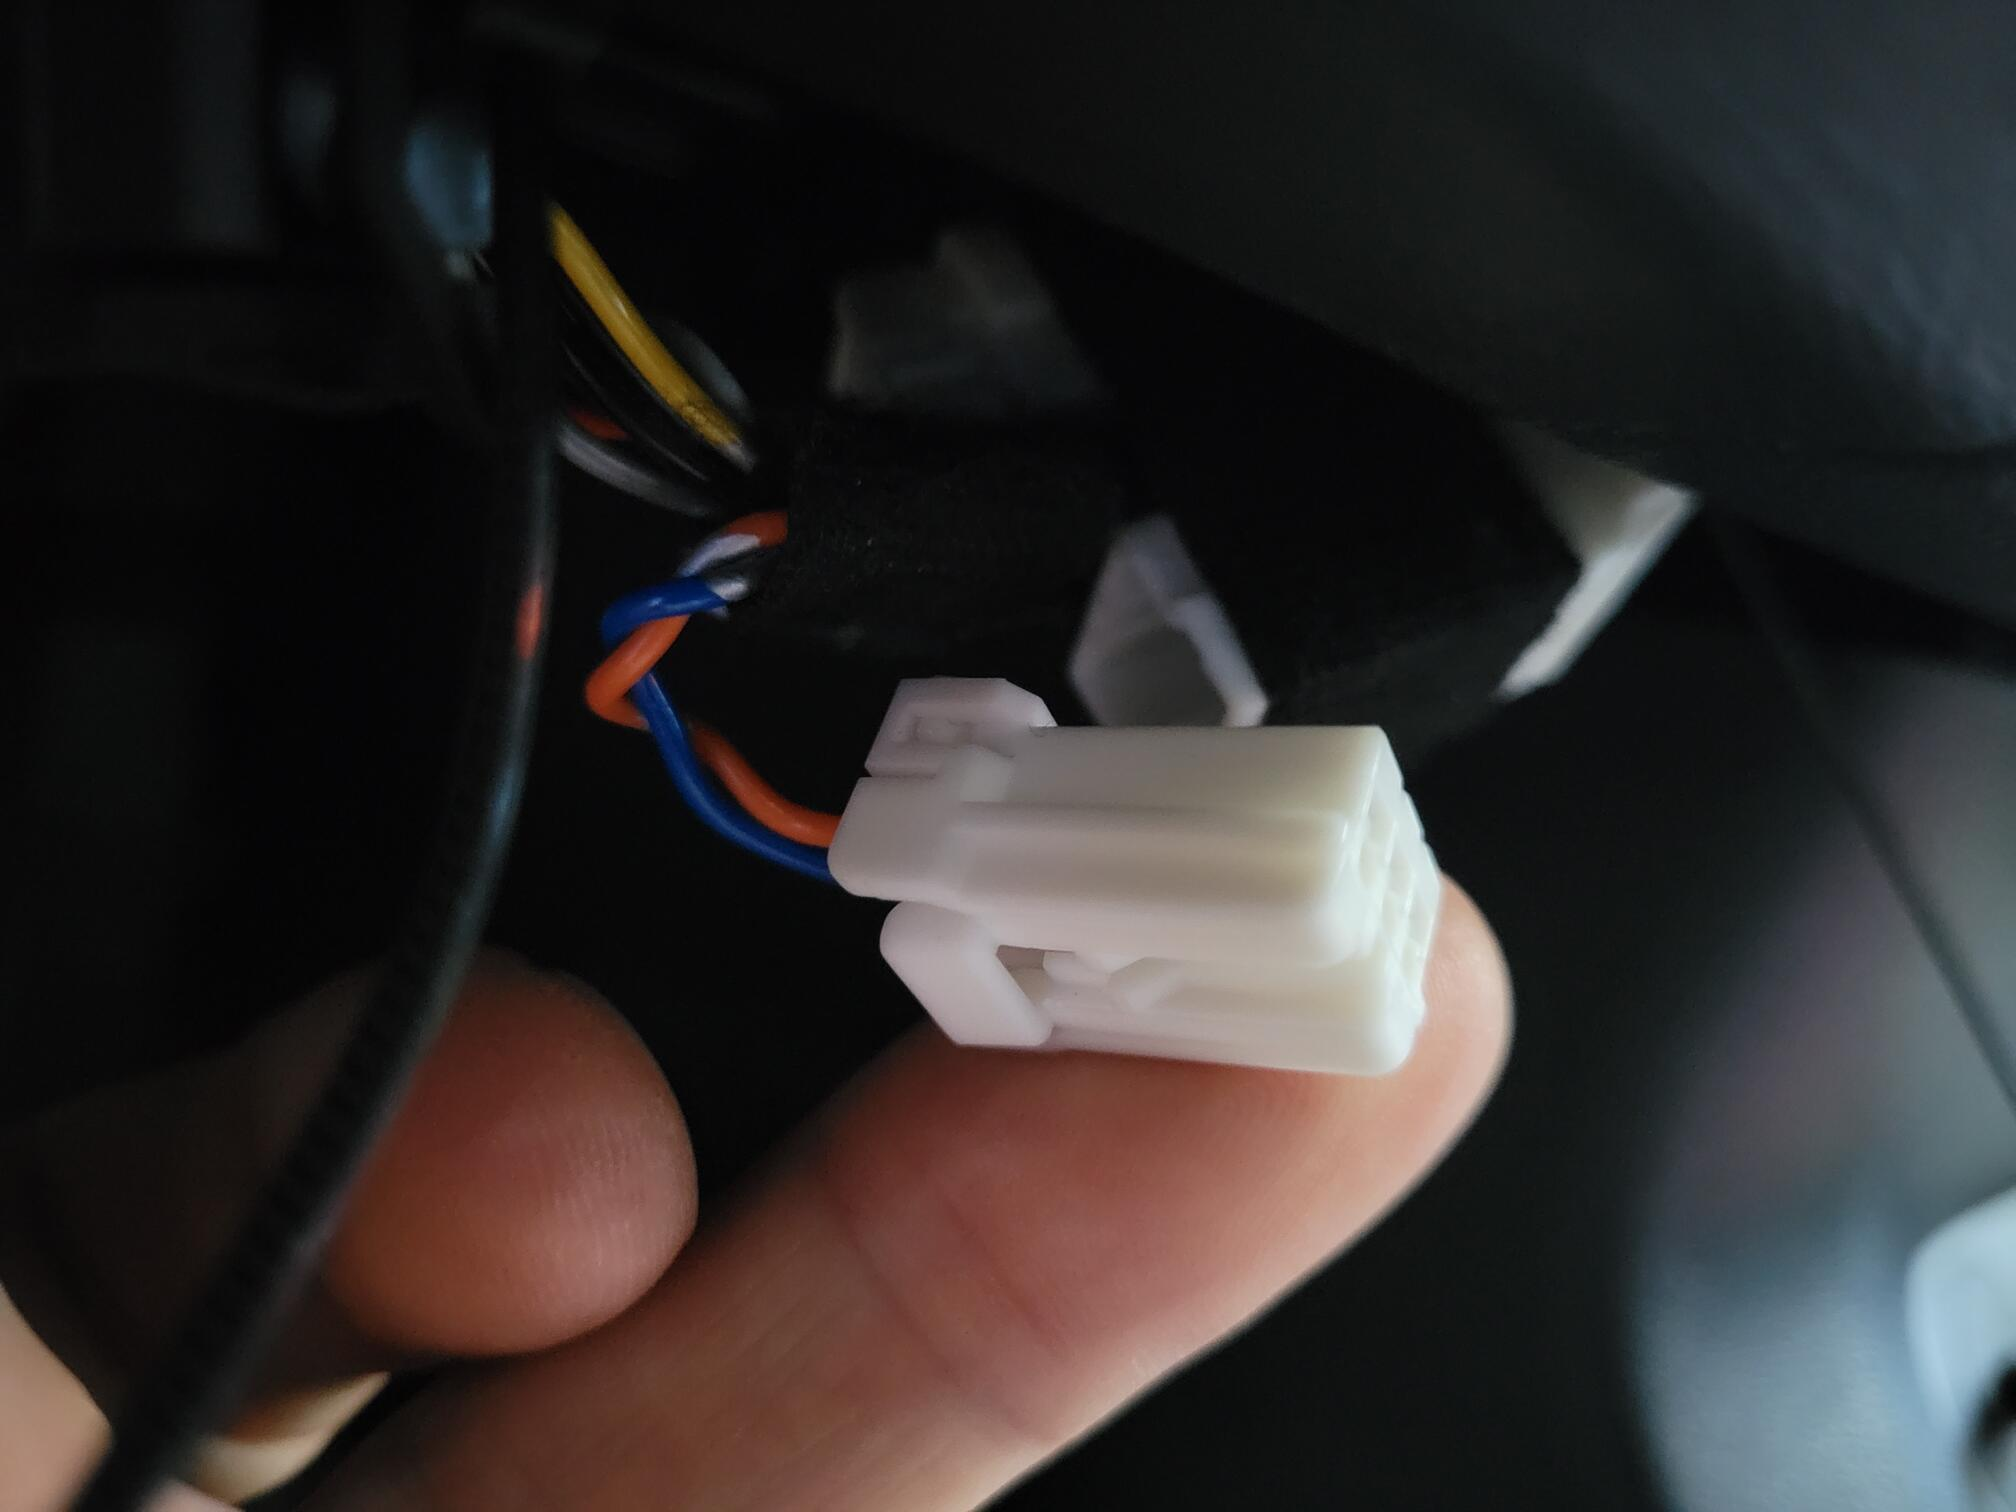
\includegraphics[height=0.95in]{photos/female_shunt_disconnected.jpg} } \\
  \subfloat[]{\label{subfig:shunt:cap_removed}
  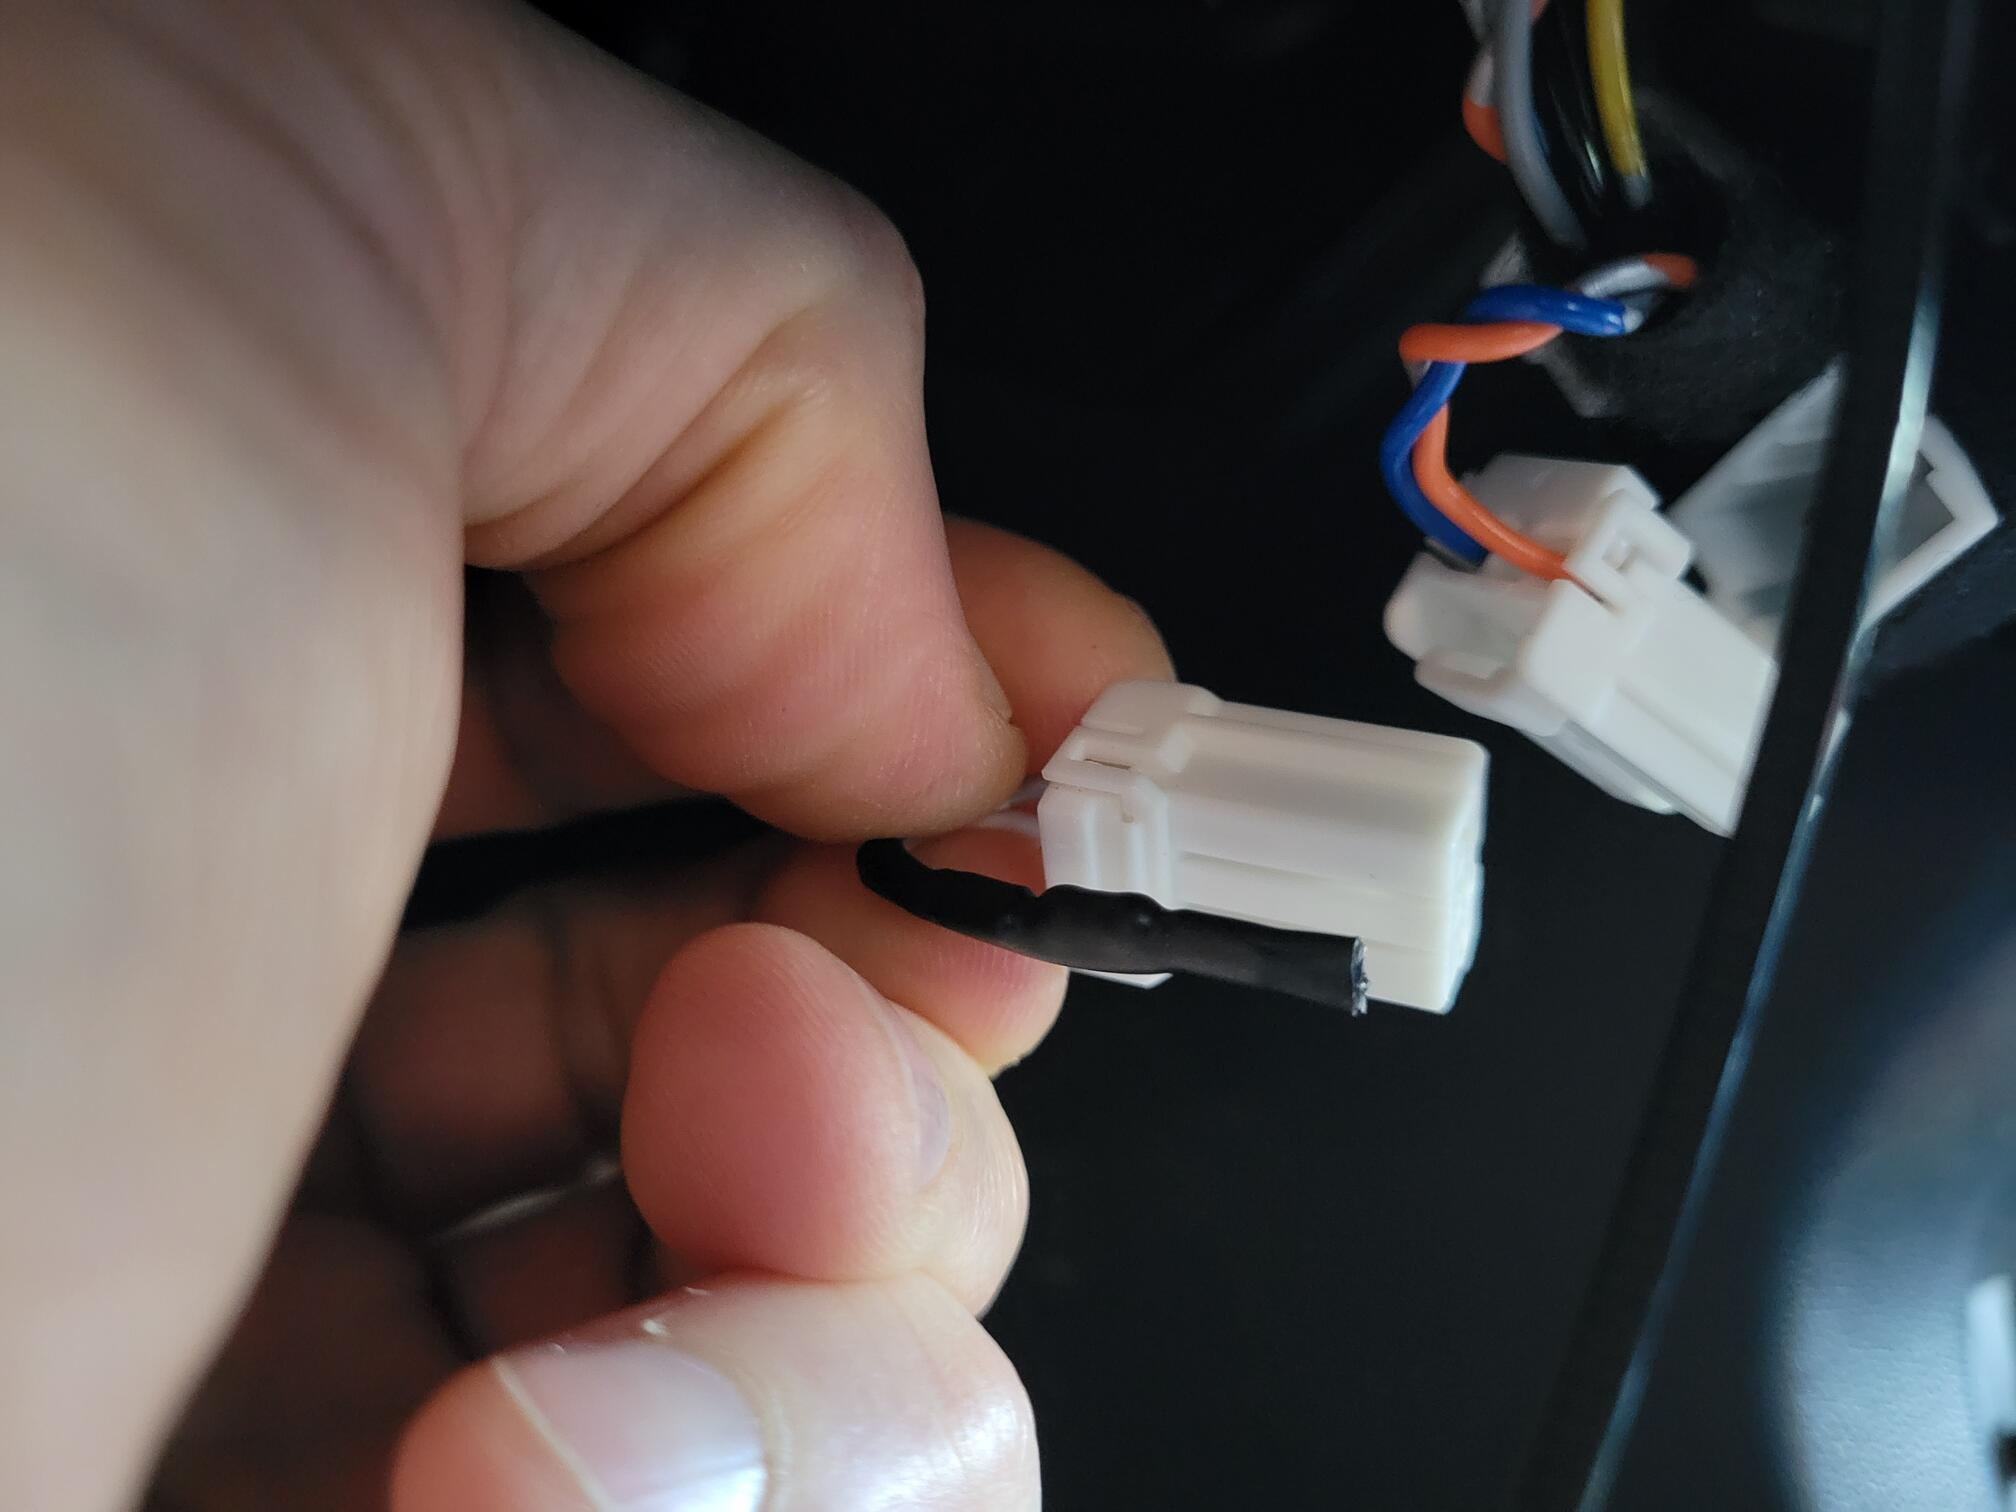
\includegraphics[height=0.95in]{photos/cap_removed.jpg} }
  \subfloat[]{\label{subfig:shunt:parallel}
  \includegraphics[height=0.95in]{photos/parallel.jpg} }
   \caption{(a-b) Capuchon de shunt femelle : MITM mpde initial. (c) Déconnexion du shunt femelle. (d) Déconnexion du capuchon de dérivation femelle. (e) Mode parallèle. \label{fig:shunts}}
\end{figure}
% %   \includegraphics[width=1.8in]{full_grating_nocblabel.png} }
% %   \begin{minipage}{1.5in}
% %     \vspace{-0.6in}
% \section{Experiment}
% 
% \begin{figure}[h]
%   \subfloat[]{\label{subfig:comparison:amp12}
%   \includegraphics[height=0.95in]{Capture12_amp_corrected_with_own_vacuum.png} }
%   \subfloat[]{\label{subfig:comparison:phase12}
%   \includegraphics[height=0.95in]{Capture12_phase_corrected_with_own_vacuum_labeled.png} }
%   \subfloat[]{\label{subfig:comparison:haadf12}
%   \includegraphics[height=0.95in]{Capture12_HAADF.png} } \\
%   \subfloat[]{\label{subfig:comparison:amp17}
%   \includegraphics[height=0.85in]{Capture17_amp_corrected_with_own_vacuum.png} }
%   \subfloat[]{\label{subfig:comparison:phase17}
%   \includegraphics[height=0.85in]{Capture17_phase_corrected_with_own_vacuum_labeled.png} }
%   \subfloat[]{\label{subfig:comparison:haadf17}
%   \includegraphics[height=0.85in]{Capture17_HAADF.png} } \\
%   \subfloat[]{\label{subfig:comparison:lacey_lineplot}
%   \includegraphics[height=1.1in]{STEMh-HAADF_comparison_lacey_carbon.png} }
%   \subfloat[]{\label{subfig:comparison:CdTe_lineplot}
%   \includegraphics[height=1.1in]{STEMh-HAADF_comparison_CdTe_noinset.png} }\\
%   \caption{Comparison of micrographs recorded by STEMH and ADF-STEM on lacey carbon and semidconducting nanoparticles. (a,d) Amplitude measured by STEMH. (b,e) Phase measured by STEMH; line profiles in (g,h) are taken along the white arrow and averaged over the width of the box. (c,f) Simultaneously acquired ADF. (g) Comparison of phase (red) with ADF (blue) on lacey carbon edge. Inset: zoom-in to show noise levels. (h) Same as (g) on the edge of a semiconducting nanoparticle. \label{fig:comparison}}%Inset: zoomed-in plot of the vacuum region just outside the particle. The phase outside the particle is fit well by an exponential decay (green). \label{fig:comparison}}
%   % starting at the edge of the particle, as determined by the maximum gradient of the ADF. 
% \end{figure}
% 
% 
\appendix 
\bibliographystyle{apsrev4-1}
\bibliography{stemh_model}{}
\end{document}